\documentclass[10pt]{article}
\usepackage[margin=1.0in]{geometry}
\usepackage{tikz,amsmath,url}
\usetikzlibrary{calc,arrows,decorations.markings,patterns}
\usepackage{parskip}

\begin{document}

\section{Warning}
I'm going to use only a physicist's level of rigour in the following.
I'm also going to assume a little familiarity with the Legendre transform and the dual of an optimisation problem.

\section{Two views of convex regions}
There are two complementary ways we can look at convex regions: in terms of the points at the boundary, or as an intersection of half planes.
The Legendre transform allows us to move back and forth between these dual representations in the case when the convex region is the {\it epigraph} of a function, the region above its graph.
(Note that we can think of a half plane as defined by a linear function on a space.
Points in the half plane are those for which the liner function evaluates to zero or less.
These linear functions are {\it duals} in the sense of linear algebra.
So the dual of convex analysis is related to that of linear algebra, despite frequent claims to the contrary.)

\section{The Legendre and Fourier transforms}
The Fourier transform also allows us to move back and forth between two representations of functions.
One is as a sum of Dirac delta functions, ie.
\[
f(x)=\int_{-\infty}^\infty dx f(a)\delta(x-a)
\]
and one is as a sum of plane waves
\[
f(x)=\frac{1}{\sqrt{2\pi}}\int_{-\infty}^\infty d\omega \hat{f}(\omega)\exp(i\omega x)
\]
The Legendre transform allows us to move between two representations in a similar way.
We can define a ``convex'' analogue of the Dirac delta function
\[
\sigma(x)=\begin{cases}
0 & x=0 \\
\infty & x\ne 0 \\
\end{cases}
\]
so we have
\[
f(x) = inf_a\, f(a)\sigma(x-a)
\]
This allows us to think of functions as infima of infinite collections of downward spikes, similar to the above picture of a function as a sum of infinitely many upward Dirac spikes.
The Legendre transform $f^\ast$ gives a function $f$ as the supremum of infinitely many straight lines:
\[
f(x) = \sup_\lambda\, (\lambda x-f^\ast(\lambda))
\]
In the case of the Fourier representation, we have a sum of plane waves, each scaled by a possibly different amount.
In the Legendre representation we have the $\sup$ of linear functions, each one shifted up or down by a possibly different amount.

There is a dictionary that allows us to translate between the language of Legendre transforms and the language of Fourier transforms.
Here is part of the dictionary:

\renewcommand{\arraystretch}{1.5}
\newcommand{\intR}{\frac{1}{\sqrt2\pi}\int_{-\infty}^{\infty}}

\begin{tabular}{| l | c | c |}
\hline

Binary operations & $+$, $\cdot$, $0$, $1$ & $\min$, $+$, $\infty$, $0$ \\

\hline

Integration & $\intR$ & $\inf$ \\

\hline

``Dirac" form & $f(x) = \intR f(p)\delta(x-p)dx$ & $f(x) = \inf_p f(p)\sigma(x-p)$ \\

\hline

Diagonalisation & $\exp(i\omega (x+a)) = \exp(i\omega a)\exp(i\omega x)$ & $p(x+a) = pa + px$ \\
& $g(x) = f(x+a)$ & $g(x) = f(x+a)$ \\
& $G(\omega) = \exp(i\omega a)F(\omega)$ & $g^\ast(p) = pa+f^\ast(p)$ \\

\hline

Fourier-Legendre transform & $F(\omega)=\intR f(x)\exp(-i\omega x)dx$ & $f^\ast(p) = \sup_x (xp-f(x))$ \\

\hline

Inverse transform & $f(x) = \intR F(\omega)\exp(i\omega x)dx$ & $f(x) = \sup_p (px-f^\ast(p))$ \\

\hline

Scaling & $g(x) = f(x+a)$ & $g(x) = f(x+a)$ \\
& $G(\omega) = \frac{1}{|a|}G(\omega/a)$ & $g^\ast(p) = f^\ast(p/a)$ \\

\hline

Unitarity/Fenchel duality & $\intR\bar{F}(\omega)G(\omega)d\omega = \intR\bar{f}(x)g(x)dx$ & $\inf_x(f(x)+g(x)) = \inf_p(f^\ast(p)+g^\ast(-p))$ \\

\hline

Plancherel's theorem & $\intR\left|F(\omega)\right|^2d\omega = \intR\left|f(x)\right|^2dx$ & $2\inf_x f(x) = \inf_p(f^\ast(p)+f^\ast(-p))$ \\

\hline

Gaussian/quadratic & $f(x) = \exp(-ax^2/2)$ & $f(x) = ax^2/2$ \\
& $F(\omega) = \frac{1}{\sqrt{a}}\exp(-\omega^2/2a)$ & $f^\ast(p) = p^2/2a$ \\

\hline

(Inf-)convolution & $h(x) = (f\otimes g)(x) = \intR f(y)g(x-y)dy$ & $h(x) = (f\oplus g)(x) = \inf_y f(y)g(x-y)$ \\
& $H(\omega) = F(\omega)G(\omega)$ & $h^\ast(p) = f^\ast(p)+g^\ast(p)$ \\

\hline

& Quantum mechanics & Classical mechanics \\

\hline

& Feynman path integral & Hamilton's principle of least action \\

\hline

\end{tabular}

my goal here is to add a couple of new entries that arise when constrained optimisation is considered.

\section{An elementary constrained optimisation}
\label{sec:opt}

\begin{figure}
\centering
\begin{tikzpicture}[
        %We set the scale and define some styles
        scale=1.5,
        axis/.style={very thick, ->, >=stealth'},
        important line/.style={thick},
        dashed line/.style={dashed, thick},
        every node/.style={color=black,}
     ]
\begin{scope}
% Important coordinates are defined
    \coordinate (l) at (0,3);
    \coordinate (b) at (2.5,0.5);
    \coordinate (c) at (5,3);
    \coordinate (a) at (3.5,0);

    %We make some nice shading to annotate different parts of the curve
    % Everything for x<0
    %  Everything for x>0
    % axis
    \draw[axis] (0,0)  -- (5.2,0) node(xline)[right] {$x$};
    \draw[axis] (0,-0.7) -- (0,3.0) node(yline)[above] {$f(x)$};
    % J curve is drawn
    \draw[important line]
        (l) parabola bend (b) (c);
    % coordinates are added
    \fill[black] (a) circle (1pt) node[below] {$a$};
    % The time of the devaluation is added
    \draw[thick,dashed] (a) -- ($(a)+(0,3)$);
\end{scope}
\end{tikzpicture}
\caption{A convex function}
\label{convex}
\end{figure}
Consider the constrained optimisation problem

\[
\begin{tabular}{l c}
minimise & $f(x)$ \\
subject to & $x\le a$ \\
\end{tabular}
\]

We can form the Lagrangian in the usual way (for example see \cite{boyd}):
\[
L(a,x,\lambda) = f(x)+\lambda(x-a) \mbox{ defined for $\lambda\ge 0$}.
\]

Minimising this with respect to $x$ gives us a new function:

\[
g(a,\lambda) = \inf_x\, (f(x)+\lambda(x-a))
\]

which gives us the dual optimisation problem:

\[
\begin{tabular}{l c}
maximise & $g(a,\lambda)$ \\
subject to & $\lambda\ge 0$ \\
\end{tabular}
\]

In this case, strong duality holds (see \cite{strong}) so both of these problems achieve the same optimal value.

Now consider the optimal value as a function of $a$, $f_+(a)=\min_{\lambda\ge0}g(a,\lambda)$.
We plot typical examples of $f(x)$ and $f_+(a)$ in Figures~\ref{convex} and \ref{min}.

\begin{figure}
\centering
\begin{tikzpicture}[
        %We set the scale and define some styles
        scale=1.5,
        axis/.style={very thick, ->, >=stealth'},
        important line/.style={thick},
        dashed line/.style={dashed, thick},
        every node/.style={color=black,}
     ]
\begin{scope}[yshift=-1.7in]
    % Important coordinates are defined
    \coordinate (l) at (0,3);
    \coordinate (b) at (2.5,0.5);
    \coordinate (c) at (5,3);

    %We make some nice shading to annotate different parts of the curve
    % Everything for x<0
    %  Everything for x>0
    % axis
    \draw[axis] (0,0)  -- (5.2,0) node(xline)[right] {$a$};
    \draw[axis] (0,-0.7) -- (0,3.0) node(yline)[above] {$f_+(a)=\min_{x\le a}f(x)$};
    % J curve is drawn
    \draw[important line]
        (l) parabola[bend at end] (b);
    \draw[important line]
        (b) -- ($(b)+(1.5,0)$);
    % coordinates are added
    % The time of the devaluation is added
\end{scope}
\end{tikzpicture}
\caption{The constrained minimum of a convex function}
\label{min}
\end{figure}

We can look at these graphs another way.
The function $f_+$ is a version of $f$ where all the parts with positive gradient have been ``removed'', keeping only the non-increasing part.
Think about this in terms of the {\it epigraph} of $f$, the set of points above the curve.
The dual view of the epigraph, illustrated in Figure~\ref{epigraph}, is that it is the intersection of an infinite collection of half-planes, each one just touching $f$.
To construct the epigraph of $f_+$ we take only those half-planes whose boundaries have non-positive gradient.
This is illustrated in Figure~\ref{epimin}.
This is precisely what the construction of the dual problem achieves.
It forms the Legendre transform of the original function.
But instead of reconstructing the original function using the full Legendre transform, instead it reconstructs it using only lines for which $\lambda\ge0$.

\begin{figure}
\centering
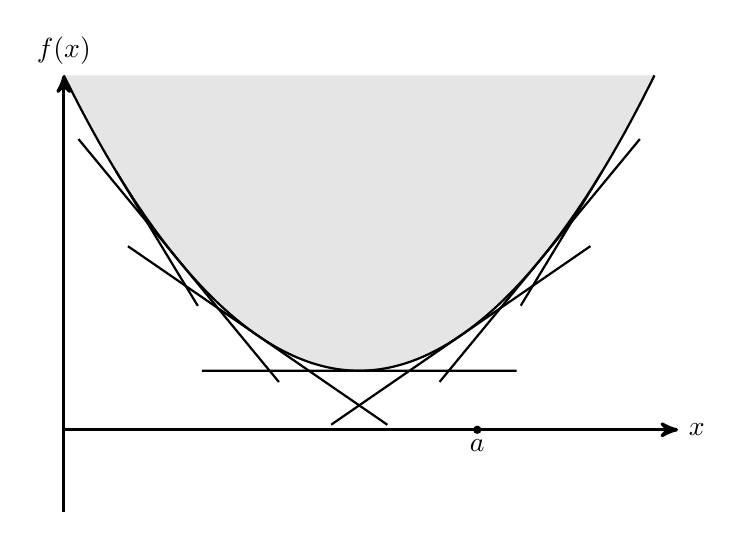
\begin{tikzpicture}[
        %We set the scale and define some styles
        scale=1.5,
        axis/.style={very thick, ->, >=stealth'},
        important line/.style={thick},
        dashed line/.style={dashed, thick},
        every node/.style={color=black,},
    tangent/.style={
        decoration={
            markings,% switch on markings
            mark=
                at position #1
                with
                {
                    \coordinate (tangent point-\pgfkeysvalueof{/pgf/decoration/mark info/sequence number}) at (0pt,0pt);
                    \coordinate (tangent unit vector-\pgfkeysvalueof{/pgf/decoration/mark info/sequence number}) at (1,0pt);
                    \coordinate (tangent orthogonal unit vector-\pgfkeysvalueof{/pgf/decoration/mark info/sequence number}) at (0pt,1);
                }
        },
        postaction=decorate
    },
    use tangent/.style={
        shift=(tangent point-#1),
        x=(tangent unit vector-#1),
        y=(tangent orthogonal unit vector-#1)
    },
    use tangent/.default=1
]
\begin{scope}
% Important coordinates are defined
    \coordinate (l) at (0,3);
    \coordinate (b) at (2.5,0.5);
    \coordinate (c) at (5,3);
    \coordinate (a) at (3.5,0);

    % axis
    \draw[axis] (0,0)  -- (5.2,0) node(xline)[right] {$x$};
    \draw[axis] (0,-0.7) -- (0,3.0) node(yline)[above] {$f(x)$};
    % J curve is drawn
    \shade[top color=black!10,bottom color=black!10]
        (l) parabola bend (b) (c);
    \draw[important line,tangent=0.125,tangent=0.25,tangent=0.375,
                         tangent=0.5,tangent=0.625,tangent=0.75,tangent=0.875]
        (l) parabola bend (b) (c);
    \draw [thick, use tangent=1] (0,0) -- (2,0);
    \draw [thick, use tangent=2] (-2,0) -- (2,0);
    \draw [thick, use tangent=3] (-2,0) -- (2,0);
    \draw [thick, use tangent=4] (-2,0) -- (2,0);
    \draw [thick, use tangent=5] (-2,0) -- (2,0);
    \draw [thick, use tangent=6] (-2,0) -- (2,0);
    \draw [thick, use tangent=7] (-2,0) -- (0,0);
    % coordinates are added
    \fill[black] (a) circle (1pt) node[below] {$a$};
    % The time of the devaluation is added
\end{scope}
\end{tikzpicture}
\caption{The epigraph of a convex function as the intersection of half-planes}
\label{epigraph}
\end{figure}

\begin{figure}
\centering
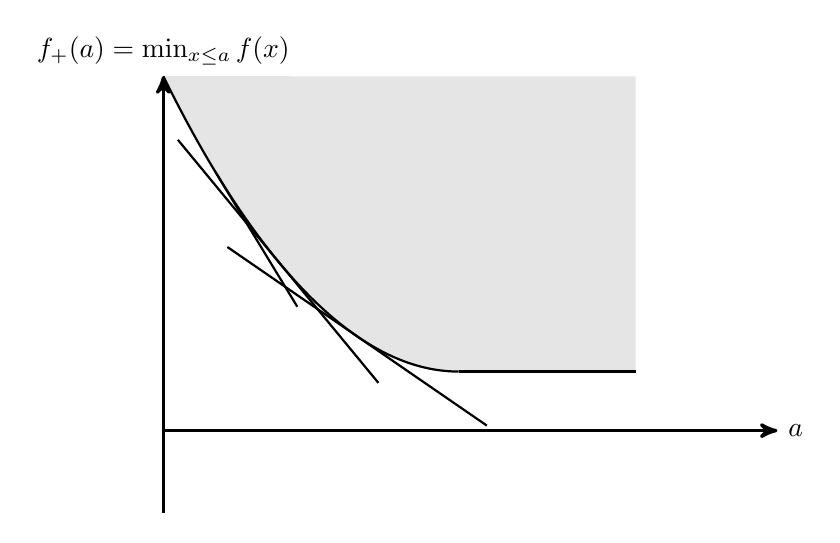
\begin{tikzpicture}[
        %We set the scale and define some styles
        scale=1.5,
        axis/.style={very thick, ->, >=stealth'},
        important line/.style={thick},
        dashed line/.style={dashed, thick},
        every node/.style={color=black,},
    tangent/.style={
        decoration={
            markings,% switch on markings
            mark=
                at position #1
                with
                {
                    \coordinate (tangent point-\pgfkeysvalueof{/pgf/decoration/mark info/sequence number}) at (0pt,0pt);
                    \coordinate (tangent unit vector-\pgfkeysvalueof{/pgf/decoration/mark info/sequence number}) at (1,0pt);
                    \coordinate (tangent orthogonal unit vector-\pgfkeysvalueof{/pgf/decoration/mark info/sequence number}) at (0pt,1);
                }
        },
        postaction=decorate
    },
    use tangent/.style={
        shift=(tangent point-#1),
        x=(tangent unit vector-#1),
        y=(tangent orthogonal unit vector-#1)
    },
    use tangent/.default=1
]
\begin{scope}[yshift=-1.7in]

    % Important coordinates are defined
    \coordinate (l) at (0,3);
    \coordinate (b) at (2.5,0.5);
    \coordinate (c) at (5,3);

    %We make some nice shading to annotate different parts of the curve
    % Everything for x<0
    %  Everything for x>0
    % axis
    \draw[axis] (0,0)  -- (5.2,0) node(xline)[right] {$a$};
    \draw[axis] (0,-0.7) -- (0,3.0) node(yline)[above] {$f_+(a)=\min_{x\le a}f(x)$};
    % J curve is drawn
    \shade[top color=black!10,bottom color=black!10]
        (l) parabola[bend at end] (b) to (4,0.5) to (4,3);
    \draw[important line,tangent=0.25,tangent=0.5,tangent=0.75]
        (l) parabola[bend at end] (b);
    \draw [thick, use tangent=1] (0,0) -- (2,0);
    \draw [thick, use tangent=2] (-2,0) -- (2,0);
    \draw [thick, use tangent=3] (-2,0) -- (2,0);
    \draw[important line]
        (b) -- ($(b)+(1.5,0)$);
    % coordinates are added
    % The time of the devaluation is added
\end{scope}
\end{tikzpicture}
\caption{The epigraph of the constrained minimum}
\label{epimin}
\end{figure}

We could have defined $f_+$ directly using the primal problem but I chose to go via the dual path to investigate what happens when we translate this to the Fourier domain.

We can also define $f_-(x)=\min_{x\ge a}f(x)$ (or similarly through a dual problem).
Our original function $f$ is now given by
\[
f(x)=\max(f_+(x),f_-(x))
\]
We've ``projected'' all of the descending bits into one function and all of the ascending bits into another.

%
% Fourier version
%
\section{The same construction in the Fourier domain}
Using the dictionary, the analogue of $f_+$ is given by
\[
g(\lambda)=\frac{1}{\sqrt{2\pi}}\int_{-\infty}^{\infty}dxf(x)\exp(-\lambda(x-a))
\]
The dual optimisation problem is now translated into
\[
I(a)=\frac{1}{\sqrt{2\pi}}\int_0^\infty d\lambda\frac{1}{\sqrt{2\pi}}\int_{-\infty}^{\infty}f(x)\exp(-\lambda(x-a))
\]

Let's swap the order of those integrals so
\[
I(a)=\frac{1}{\sqrt{2\pi}}\int_{-\infty}^{\infty}f(x)\frac{1}{\sqrt{2\pi}}\int_0^\infty d\lambda\exp(-\lambda(x-a))
\]

The $\lambda$ integral is essentially the Fourier transform of the Heaviside theta function \cite{htheta}.
If
\[
\Theta(x) = \begin{cases}
0 & \mbox{ if }x<0 \\
1 & \mbox{ if }x\ge 0 \\
\end{cases}
\]
then
\[
\hat{\Theta}(\lambda)=\sqrt{\frac{\pi}{2}}\delta(\lambda)-\frac{i}{\sqrt{2\pi}(x-a)}
\]
That expression is to be interpreted as a distribution so it needs to be evaluated in an integral. The $\frac{1}{\lambda}$ requires the principal part of the integral.
We get
\[
I(a)=\frac{1}{2}f(x)+\frac{i}{2\pi}P\!\int_{-\infty}^\infty\frac{f(x)dx}{a-x}
\]
with $P\!\int$ being the principal part of the integral.
We can write this as
\[
I(a) = \frac{1}{2}f(x)+i\frac{1}{2}Hf(x)
\]
where $H$ is the Hilbert transform \cite{hilbert}.
The Hilbert transform is used to solve a certain type of Riemann-Hilbert \cite{rh} problem.
This is the problem of taking a function $f$ on the real line and writing it as
\[
f(x)=F_+(x)-F_-(x)
\]
with $F_+$ holomorphic (ie. analytic with no poles) on the upper half plane (UHP) and $F_-$ holomorphic on the lower half plane (LHP).
In fact
\[
F_+(x) = \frac{1}{2}f(x)+\frac{i}{2}Hf(x)
\]
Compare with the end of Section~\ref{sec:opt}.
Both versions allow us to ``project'' functions onto a pair of subspaces.
In the first case it was non-increasing and non-decreasing functions.
In the second case it was functions without poles in the upper half plane and functions without poles in the lower half plane.
That suggests adding these two rows to the dictionary:

\begin{tabular}{| l | l |}
\hline

Non-increasing convex functions & functions whose analytic continuation to the UHP has no poles \\

\hline

Non-decreasing convex functions & functions whose analytic continuation to the LHP has no poles \\

\hline
\end{tabular}

\section{Notes}
I plan to finish this document one day.
When I do, here are some things I'll mention:

The analogy quantum-classical mechanics isn't quite perfect.
If the Lagrangian is quadratic then Hamilton's principle is a convex optimisation with a unique local minimum.
However, more general physics problems aren't convex and we need to consider all stationary solutions, minima and saddle points included.
The analogy works slightly differently in these cases.

Laplace transforms are closely related to Fourier transforms and this means we also have a Laplace-Legendre dictionary too.
This is why the Legendre transform arises in thermodynamics.

There are some ``operations'' that take us between the two domains.
For example Maslov dequentization.
And the stationary phase approximation.

I learnt about this stuff from John Baez but haven't decided on the best reference to give.

\section{Summary}
Forming the dual to an optimisation constrained by an inequality, and computing the Hilbert transform, are almost the related operations.
In one case we form the Legendre transform, throw away ``half'' of the result and then invert the Legendre transform.
In the other we do something similar with the Fourier transform.

\bibliographystyle{plain}
\bibliography{legendre}

\end{document}
